The N-Queens puzzle is the problem of placing N chess queens on an NxN
chessboard so that no pair of two queens attack each other~\cite{8queens}. The
specific challenge of finding all the distinct solutions to this problem is a
good benchmark in designing parallel algorithms.  Most popular parallel
implementations of the N-Queens problem distribute the search space of the
problem by assigning incomplete boards as tasks to threads.  Our approach is
unusual since the squares of the board as the tasks of program.
Figure~\ref{code:coordination:nqueens} presents our solution.


N Queens nodes are the squares of the chessboard and each square can communicate
with other 4 squares: the adjacent right and the adjacent left on the same row,
and the first non-diagonal square to the right and to the left on the row below.
To represent a partial/valid board state, we use a list of integers, where each
pair of integers represents a coordinate in which a queen is placed. For example
$[1, 2, 0, 0]$ means that a queen is placed in square $(0, 0)$ and another in
square $(1, 2)$. At any given time, many partial states can be using the same
squares.  Each square can also have many states at the same time.

\begin{figure}[ht!]
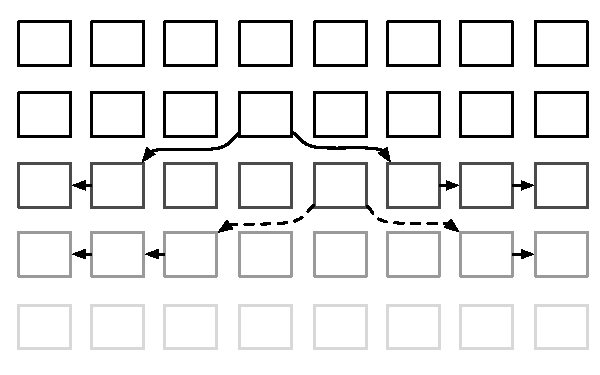
\includegraphics[width=0.4\textwidth]{figures/coordination/nqueens.pdf}
\caption{Concurrent propagation of N-Queens states.}
\label{coordination:fig:nqueens}
\end{figure}

An empty state is instantiated in the top-left square
(line~\ref{line:coord:queens_axiom}) and is then propagated to all squares in
the same row (rule in
lines~\ref{line:coord:queens_propr1}-\ref{line:coord:queens_propr2}). Once a
square $S$ receives a new state $L$, it checks if $S$ can be incorporated into
$L$. For that, it checks if there is no queen on $S$'s column (rules in lines
\ref{line:coord:queens_col1}-\ref{line:coord:queens_col2}), if there is no queen
on $S$'s left diagonal (rules in
lines~\ref{line:coord:queens_ldiag1}-\ref{line:coord:queens_ldiag2}) and if
there is no queen on $S$'s right diagonal (rules in
lines~\ref{line:coord:queens_rdiag1}-\ref{line:coord:queens_rdiag2}).

If there is any conflict, we do not derive anything and for that we use the
language expression \code{1}
(lines~\ref{line:coord:queens_empty1},~\ref{line:coord:queens_empty2}
and~\ref{line:coord:queens_empty3}), which corresponds to an empty rule head. If
there are no conflicts, this means that it is possible to add a queen to the
current state (line~\ref{line:coord:queens_add}). The fact \code{send-down/2} is
used to either complete the computation of a valid state
(lines~\ref{line:coord:queens_complete1}-\ref{line:coord:queens_complete2}) or
to propagate the state to the row below
(lines~\ref{line:coord:queens_down1}-\ref{line:coord:queens_down2}) as shown in
Fig.~\ref{coordination:fig:nqueens}.

Since computation goes from the top row to the bottom row, not all static
placements of nodes to threads will perform equally well. This is especially
true because the bottom rows tend to perform the most work.  The best placement
is then to split the board vertically with axiom \code{set-thread(A, vertical(X,
Y))} so each thread gets the same number of columns, where \code{X} and \code{Y}
are the coordinates of a particular square. Our experiments show that, on a
shared memory system, it does not matter much if we start with a bad placement
since node stealing overcomes those issues by load balancing dynamically.
However, the N Queens program incrementally builds and shares lists representing
valid board states that are transmitted from top to bottom. In order to improve
memory locality we should then manipulate board states that share a significant
number of elements because each board state needs to be iterated before being
extended with a new position. To accomplish this, we used the coordination fact
\code{set-default-priority(A, X)} to experiment with two configurations:
\code{Top}, where top rows are prioritized; and \code{Bottom}, where squares
closer to the bottom are computed first. We also decided to optionally pin nodes
to threads, as mentioned earlier, to see if memory locality affects the
multi-threaded performance of the program.

%% XXX results
\begin{figure}[h!]
\begin{Verbatim}[numbers=left,fontsize=\scriptsize,commandchars=\*\#\&]
type list int state.
type left(node, node).  type right(node, node).
type down-left(node, node).  type down-right(node, node).
type coord(node, int, int).
type linear propagate-left(node, state).
type linear propagate-right(node, state).
type linear test-y(node, int, state, state).
type linear test-diag-left(node, int, int, state, state).
type linear test-diag-right(node, int, int, state, state).
type linear send-down(node, state).
type linear new-state(node, state).
type linear final-state(node, state).

propagate-right(@0, []).*label#line:coord:queens_axiom&

propagate-left(A, State)
  -o {L | !left(A, L), L <> A | propagate-left(L, State)}, new-state(A, State).
propagate-right(A, State)*label#line:coord:queens_propr1&
  -o {R | !right(A, R), R <> A | propagate-right(R, State)}, new-state(A, State).*label#line:coord:queens_propr2&

new-state(A, State), !coord(A, X, Y) -o test-y(A, Y, State, State).

// check if there is no queen on the same column*label#line:coord:queens_col1&
test-y(A, Y, [], State), !coord(A, OX, OY)
  -o test-diag-left(A, OX - 1, OY - 1, State, State).
test-y(A, Y, [X, Y1 | RestState], State), Y = Y1
  -o 1. // fail*label#line:coord:queens_empty1&
test-y(A, Y, [X, Y1 | RestState], State), Y <> Y1
  -o test-y(A, Y, RestState, State).*label#line:coord:queens_col2&

// check if there is no queen on the left diagonal*label#line:coord:queens_ldiag1&
test-diag-left(A, X, Y, _, State), X < 0 || Y < 0, !coord(A, OX, OY)
  -o test-diag-right(A, OX - 1, OY + 1, State, State).
test-diag-left(A, X, Y, [X1, Y1 | RestState], State), X = X1, Y = Y1
  -o 1. // fail*label#line:coord:queens_empty2&
test-diag-left(A, X, Y, [X1, Y1 | RestState], State), X <> X1 || Y <> Y1
  -o test-diag-left(A, X - 1, Y - 1, RestState, State).*label#line:coord:queens_ldiag2&

// check if there is no queen on the right diagonal*label#line:coord:queens_rdiag1&
test-diag-right(A, X, Y, [], State), X < 0 || Y >= size, !coord(A, OX, OY)
  -o send-down(A, [OX, OY | State]). // add new queen*label#line:coord:queens_add&
test-diag-right(A, X, Y, [X1, Y1 | RestState], State), X = X1, Y = Y1
  -o 1. // fail*label#line:coord:queens_empty3&
test-diag-right(A, X, Y, [X1, Y1 | RestState], State), X <> X1 || Y <> Y1
  -o test-diag-right(A, X - 1, Y + 1, RestState, State).*label#line:coord:queens_rdiag2&

send-down(A, State), !coord(A, size - 1, _)*label#line:coord:queens_complete1&
  -o final-state(A, State).*label#line:coord:queens_complete2&
send-down(A, State), !coord(A, CX, _), CX <> size - 1*label#line:coord:queens_down1&
  -o {B | !down-right(A, B), B <> A | propagate-right(B, State)},
     {B | !down-left(A, B), B <> A | propagate-left(B, State)}.*label#line:coord:queens_down2&
\end{Verbatim}
  \caption{N-Queens problem solved in LM.}
  \label{code:coordination:nqueens}
\end{figure}


\subsubsection{Proof Of Correctness}

\begin{lemma}[test-y lemma]

If \code{test-y(A, Y, State, OriginalState)} then either $\exists_{x'}. {(x',
y) \in \mathtt{State}}$ and \code{test-y} is consumed or
\code{test-diag-left(A, OX - 1, OY - 1, OriginalState, OriginalState)}, where
\code{OX} and \code{OY} are the coordinates of the square.

\end{lemma}
\begin{proof}
Induction on the size of \code{State}.

First rule: immediately the second conclusion.

Second rule: immediately the third conclusion.

Third rule: by induction.
\end{proof}

\begin{lemma}[test-diag-left lemma]
If \code{test-diag-left(A, X, Y, State, OriginalState)} then either $\exists_{x', y'}. {(x', y') \in \mathtt{State}}$, where $x = x' - a$ and $y' = y - a$, where $a$ is positive or $0$ and \code{test-diag-left} is consumed or \code{test-diag-right(A, OX - 1, OY + 1, OriginalState, OriginalState)}, where \code{OX} and \code{OY} are the coordinates of the square.
\end{lemma}
\begin{proof}
Induction on the size of \code{State}.

First rule: immediately the second conclusion.

Second rule: immediately the first conclusion.

Third rule: by induction.
\end{proof}

\begin{lemma}[test-diag-right lemma]
If \code{test-diag-right(A, X, Y, State, OriginalState)} then either $\exists_{x', y'}. {(x', y') \in \mathtt{State}}$, where $x = x' - a$ and $y' = y + a$, where $a$ is positive or $0$ and \code{test-diag-right} is consumed or \code{send-down(A, [(OX, OY) | OriginalState])}, where \code{OX} and \code{OY} are the coordinates of the square.
\end{lemma}
\begin{proof}
Induction on the size of \code{State}.

First rule: immediately the second conclusion.

Second rule: immediately the first conclusion.

Third rule: by induction.
\end{proof}

\begin{theorem}[State validation]
If \code{test-y(A, OY, State, State)} then either everything is consumed or \code{send-down(A, [(OX, OY) | State])} is derived, where \code{OX} and \code{OY} are the coordinates of the square and are a valid addition to the \code{State}.
\end{theorem}
\begin{proof}
Use the previous three lemmas.
\end{proof}

\begin{lemma}[Propagate left lemma]
If \code{propagate-left(A, State)} then every cell to the left, including \code{A} will derive \code{new-state(A, State)}.
\end{lemma}
\begin{proof}
By induction on the number of cells to the left of \code{A}. The only rule that uses \code{propagate-left/2} will prove the lemma.
\end{proof}

\begin{lemma}[Propagate right lemma]
If \code{propagate-right(A, State)} then every cell to the right, including \code{A} will derive \code{new-state(A, State)}.
\end{lemma}
\begin{proof}
By induction on the number of cells to the right of \code{A}. The only rule that uses \code{propagate-right/2} will prove the lemma.
\end{proof}

\begin{theorem}[States theorem]
For a given row, we will compute several \code{send-down(A, State)} facts that represent valid configurations that include that row and the rows above.
\end{theorem}
\begin{proof}
By induction on the number of rows.

For row 0, we use the axiom \code{propagate-right(@0, [])}, that will be propagated to all nodes in row 0. By using the state validation theorem, we know that every node will derive \code{send-down(A, [(X, Y)])}, all valid configurations.


By induction, we know that row $X'$ has derived every \code{send-down/2} possible. Such facts will be sent downwards to row $X = X' + 1$ using the last rule in the program, deriving \code{propagate-right} or \code{propagate-left} that will derive \code{new-state} at each right or left cell. We do not derive anything at the cell below or the ones to the sides since they would not be valid. Using the \code{new-state} fact, we get a \code{test-y} fact that will be checked using the state validation theorem, filtering all new valid configurations and deriving \code{send-down/2}.
\end{proof}

\clearpage
